\section{Respostas dos exercícios}

\begin{frame}[allowframebreaks]{Respostas dos exercícios}
    \begin{enumerate}
        \item São funções: $c$ e $d$.
        
        \item São funções: $a, d$ e $e$.
        
        \item 
        \begin{enumerate}[a]
            \item $-(x-1)$
            \item $-2x-h+2$
        \end{enumerate}

        \item 
        \begin{enumerate}[a]
            \item $D(f) = \conj{-3, -2, -1, 0, 1, 2, 3}$ e $Im(f) = \conj{1, 2, 3, 4, 5}$
            \item $D(f) = [-2, 3]$ e $Im(f) = [-3, 2]$
            \item $D(f) = [-2, 4]$ e $Im(f) = [1, 5]$
            \item $D(f) = [-3, 5)$ e $Im(f) = [1, 3)$
            \item $D(f) = [-4, 4]$ e $Im(f) = [-3, 5]$
            \item $D(f) = [-3, 4)$ e $Im(f) = \conj{-3, -2, -1, 0, 1, 2, 3}$
        \end{enumerate}

        \vspace{1cm}

        \item $D(f) = \R$ e $Im(f) = {-3}$

        \begin{figure}
        \centering
        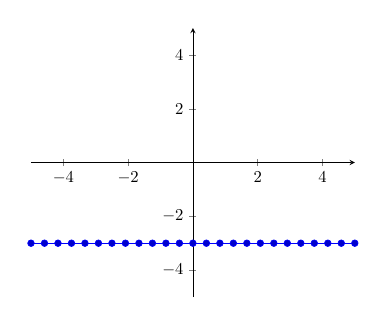
\begin{tikzpicture}[scale=0.6]
        \begin{axis}[xmin=-5, xmax=5, ymin=-5, ymax=5, axis lines=middle]
            \addplot{-3};
        \end{axis}
        \end{tikzpicture}
        \caption{$f(x) = -3$}
        \end{figure}

        \skipframe

        \item $D(f) = \R$ e $Im(f) = [0, \infty)$

        \begin{figure}
        \centering
        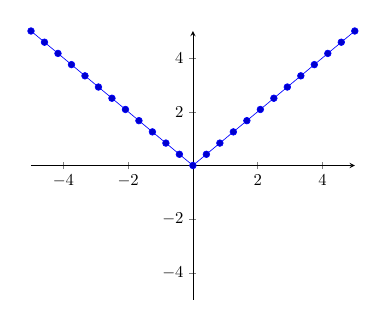
\begin{tikzpicture}[scale=0.6]
        \begin{axis}[xmin=-5, xmax=5, ymin=-5, ymax=5, axis lines=middle]
            \addplot{abs(x)};
        \end{axis}
        \end{tikzpicture}
        \caption{$f(x) = \abs{x}$}
        \end{figure}

        \item <colocar gráficos>

        \skipframe

        \item $D(f) = [-2, 6)$ e $Im(f) = [-2, 4]$

        \item $D(f) = [3, \infty) - {5}$

        \item $(1/2, \infty)$

        \skipframe

        \item $D(f) = (-\infty, \infty) - {5}$ e $Im(f) = [-1, \infty)$. O gráfico de $f$ corresponde ao do valor absoluto deslocado duas unidades para a direita e uma unidade verticalmente.

        \vspace{0.5cm}

        \begin{figure}
        \centering
        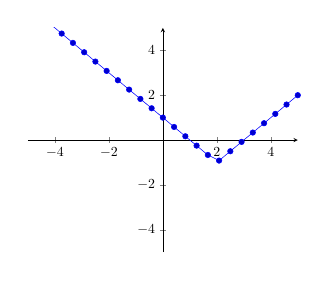
\begin{tikzpicture}[scale=0.5]
        \begin{axis}[xmin=-5, xmax=5, ymin=-5, ymax=5, axis lines=middle]
            \addplot{abs(x-2)-1};
        \end{axis}
        \end{tikzpicture}
        \caption{$f(x) = \abs{x-2}-1$}
        \end{figure}

        \skipframe

        \item 
        \begin{enumerate}[a]
            \item Posição 4.
            \item Posição 1.
            \item Posição 2.
            \item Posição 3.
        \end{enumerate}

        \item

        \item 
        \begin{enumerate}[a]
            \item 2
            \item 22
            \item $x^2 + 2$
            \item $x^2 + 10x + 22$
            \item 5
            \item -2
            \item $x + 10$
            \item $x^4 - 6x^2 + 6$
        \end{enumerate}

        \item 
        \begin{multicols}{2}
            \begin{enumerate}[a]
                \item $\dfrac{4}{x^2} - 5$
                \item $\dfrac{4}{x^2} - 5$
                \item $\parenthesis{\dfrac{4}{x} - 5}^2$
                \item $\parenthesis{\dfrac{1}{4x-5}}^2$
                \item $\dfrac{1}{4x^2 - 5}$
                \item $\dfrac{1}{(4x-5)^2}$
            \end{enumerate}
        \end{multicols}

        \skipframe

        \item
            \begin{enumerate}[a]
                \item $(f \circ g)(x) = f(g(x)) = \sqrt{x+1}$ e $D(f \circ g) = [-1, \infty)$
                \item $(g \circ f)(x) = g(f(x)) = \sqrt{x}+1$ e $D(g \circ f) = [0, \infty)$
                \item $(f \circ f)(x) = f(f(x)) = \sqrt{\sqrt{x}}$ e $D(f \circ f) = [0, \infty)$
                \item $(g \circ g)(x) = g(g(x)) = x+2$ e $D(g \circ g) = (-\infty, \infty)$
            \end{enumerate}

        \item 
        \begin{multicols}{2}
            \begin{enumerate}[a]
                \item $\dfrac{x-3}{2}$
                \item $\dfrac{3x+1}{4}$
                \item $\sqrt[3]{x-2}$
                \item $1 + \sqrt[3]{x-2}$
                \item $x^3 - 2$
                \item $(x+1)^3$
                \item $\sqrt[3]{1-x^3}$
            \end{enumerate}
        \end{multicols} 

        \skipframe

        \item $(g \circ f)^{-1}(x) = (f^{-1} \circ g^{-1})(x) = (f^{-1} \circ g^{-1})(x) = f^{-1}(g^{-1}(x)) = \dfrac{x-1}{6}$

        \item $(g \circ f)^{-1}(x) = \sqrt[3]{\dfrac{x-3}{2}}$

        \item 
        \begin{enumerate}[a]
            \item $f^{-1}(x) = \log_2 (x-3) + 1$

            \item $h(1/4) = 0$. Resolução:
            \begin{align*}
                f(h(x)) &= 3 + 2x \\
                f^{-1}(f(h(x))) &= f^{-1}(3 + 2x) \\
                h(x) &= \log_2 (3 + 2x - 3) + 1 \\
                h(x) &= \log_2 (2x) + 1 \\
                h(x) &= \log_2 (2) + \log_2 (x) + 1 \\
                h(x) &= \log_2 (x) + 2 \\
                h(x) &= \log_2 (1/4) + 2 \\
                h(x) &= -2 + 2 = 0 \\
            \end{align*}
        \end{enumerate}

        \item 
        \begin{multicols}{2}
            \begin{enumerate}[a]
                \item $a = -2$ (decrescente) e $\frac{1}{2}$
                \item $a = 5$ (crescente) e $\frac{2}{5}$
                \item $a = 3$ (crescente) e 0
                \item $a = -6$ (decrescente) e 0
                \item $a = 0$ (crescente) e o zero da função não existe
            \end{enumerate}
        \end{multicols} 

        \item $D(f) = [0, \infty)$ e $Im(f) = [0, 1]$

        \begin{equation*}
            f(x) = \begin{cases}
                        x, &\quad \text{se } 0 \leq x \leq 1 \\
                        2-x, &\quad \text{se } 1 < x \leq 2 \\
                        0, &\quad \text{se } x > 2 \\
                   \end{cases}
        \end{equation*}

        \item 

        \item Crescente para $m > 1$; decrescente para $m < 1$ e constante ($y=2$) para $m=1$.

        \item $k < -1$

        \item $A = (-0.4495,0)$, $B = (4,4495,0)$ e $C = (2,3)$

        \item $m = -2$ ou $m = 1$

        \item
        \begin{enumerate}[a]
            \item Função polinomial de grau 3 (função cúbica)
            \item \begin{figure}[h]
                    \centering
                    \begin{tikzpicture}[scale=0.6]
                    \begin{axis}[xmin=-100, xmax=100, ymin=-100, ymax=100, axis lines=middle]
                        \addplot{15/100 + x/2 + (5(x^2)/100) + ((x^3)/1000)};
                    \end{axis}
                    \end{tikzpicture}
                  \end{figure}
            \item 1550,15
            \item 0,15
            \item Aproximadamente 48 unidades (tente pelo gráfico)
        \end{enumerate}
        
    \end{enumerate}
\end{frame}